\documentclass[sigconf,nonacm]{acmart}
%% \BibTeX command to typeset BibTeX logo in the docs
\AtBeginDocument{%
  \providecommand\BibTeX{{%
    \normalfont B\kern-0.5em{\scshape i\kern-0.25em b}\kern-0.8em\TeX}}}

\begin{document}


\title{CS145 Team 22 Midterm Report}

\author{Hamlin Liu}
\affiliation{%
  \institution{UCLA, 805103522}
  }
\email{hamlin.liu@gmail.com}

\author{Shriniket Buche}
\affiliation{%
  \institution{UCLA, 305088562}
  }
\email{shriniketbuche@gmail.com}

\author{Juan Estrada}
\affiliation{%
  \institution{UCLA, 105347991}
  }
\email{juanestrada@ucla.edu}

\author{Yash Lala}
\affiliation{%
  \institution{UCLA, 905159212}
  }
\email{yashlala@gmail.com}

\author{Justin Yi}
\affiliation{%
  \institution{UCLA, 905123893}
  }
\email{joostinyi00@gmail.com}

\renewcommand{\shortauthors}{Team 22}

%% A short summary of the work to be presented.
\begin{abstract}
COVID-19, the theme of our CS 145 project, has been classified as a worldwide
pandemic. The rate of its spread is a complex function of local social
distancing, government policy, climate, and many other factors. Detailed
analysis of all of these contributory causes is not humanly possible. However,
we can build reasonably accurate disease models by using the Data Mining
techniques taught in CS 145. This report documents our team’s efforts towards
analyzing COVID-related data in the month of September. We catalogue our
initial data explorations, our efforts towards data regularization, and our
future predictions as we construct a model capable of predicting fatalities
caused by COVID-19. 
\end{abstract}

\maketitle

\section{Exploratory Data Analysis}

To begin designing the model for COVID Prediction, we decided to do some
exploratory data analysis (EDA) to visualize any patterns or trends that we
could leverage to increase the accuracy of our model. The dataset itself mainly
consisted of the daily COVID-19 statistics of each state from early April to
the end of August.

Some first observations that were noticed were the inconsistencies from state
by state. Hospitalization records and recovered count varied state by state.
Thus these statistics would probably only work if the models were trained on
each state specifically. In addition, nationally, the trends of each state
varied drastically mostly due to the varying population sizes of each state.
This can be seen with the first 20 states in alphabetical order figure and
their confirmed cases throughout the months of April and August.

\begin{figure}
  \centering
  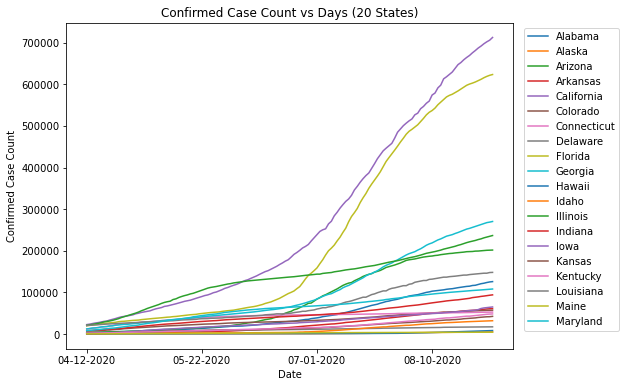
\includegraphics[width=\linewidth]{national-trends.png}
  \caption{Confirmed Cases in Various States}
\end{figure}

However, once we separate each state by itself, we start to see some more
obvious patterns. The geographic location of each state seemed to be a major
factor in the pattern of confirmed cases of each state. For example, comparing
Connecticut, New York, and New Jersey, (shown below), they had somewhat of a
logistic curve in the beginning, though the rate at which the cases were
increasing were much different compared to each other. The same can be applied
to Oregon, Washington, and California, the three states that border the
Pacific. 

\begin{figure}
  \centering
  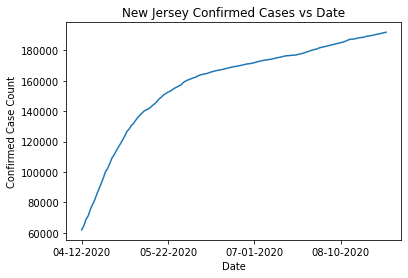
\includegraphics[width=\linewidth]{new-jersey-cases.png}
  \caption{Confirmed Cases in New Jersey}
\end{figure}

\begin{figure}
  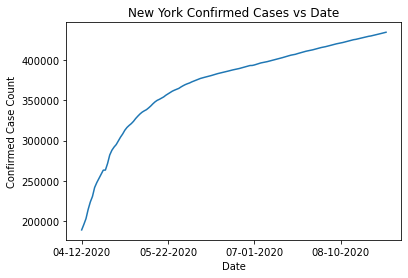
\includegraphics[width=\linewidth]{new-york-cases.png}
  \caption{Confirmed Cases in New York}
\end{figure}

\begin{figure}
  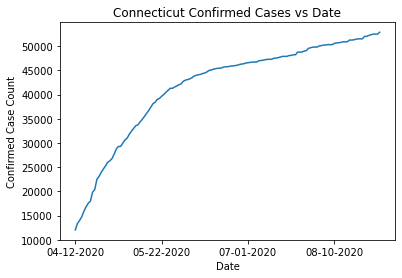
\includegraphics[width=\linewidth]{connecticut-cases.png}
  \caption{Confirmed Cases in Connecticut}
\end{figure}

Thus from the initial observations, we can see that a general model of the
United States might not work as well as models that are specific to each state
as well as including some type of way to include the geographical location into
our training. The main conclusion we found was the need for preprocessing,
first to normalize the data by state and second to try and remove some empty
periods in the data collection.

\section{Data Preprocessing}

Now moving on to actually wrangling the data for processing and straightforward
input to our prospective models, we first needed to examine the existing data
to analyze where help was needed. Upon inspection of data types, it is noted
that much of our data is numerical, bar the categorical and ordinal columns of
Province\_State and Date, respectively. We chose to convert the date from a
string type to datetime object type, to ease future parsing. Using our
contextual knowledge of our problem space, we chose to address the modeling
problem from an individual Province\_State perspective, i.e. we grouped our
data by the Province\_State field. From here on, we will refer to this
“Province\_State” field simply as the “state”. 

Our initial imputation strategy went as follows: 
We examined each state’s numeric data column by column. If null values
comprised more than 70\% of the total data in the column, we dropped the entire
column; otherwise, we replaced all null values with the median value in our
column. 
After noting that this approach led to “plateaus” in our data, we tried
linearly interpolating the values in each column. This approach produces more
organic data in each column, but fails to impute data at the beginning of a
time series (due to having no “base point” to interpolate off of). Because our
current models treat every column separately, we don’t anticipate that this
will cause issues; we can drop NaN values to create new “columns” that are
perfectly interpolated, but start at a later date.  

After interpolating the data, we normalized it to zero mean unit variance. At
this time, we are still considering whether to normalize the data globally or
within a single column. Intuition would suggest that a column-wise approach
would be best.

\section{Prototyping}

As we initially saw from the observations of the data, creating a tailored
model per state will probably lead to better results as the trend for each
state varies from more populous states to less populous ones. Initially we
tried a linear regression model using scikit-learn \cite{scikit-learn}, using
parameters such as the number of active cases, incident rate etc. 

The 1st model with a regular linear regression was trained on all the features
and data points. This model performed poorly with a MAPE of 5.8 on the
leaderboard data. There are multiple reasons for the poor performance. Some of
the few are that the confirmed cases and death numbers aren't linear, and there
is lag time before cases and deaths begin to rise. To combat this we designed a
model that only used the last 40 days of the data. This makes sure that all the
data is after the initial increase in cases and deaths. This model performed
much better than our first model achieving a MAPE of 3.3 on the leaderboard
data. We concluded that a purely linear regression model might be just good
enough to beat the benchmark, but would not be viable to push further than
that.  Also while we could validate this data with our training data, there was
simply no way of predicting future cases as the input parameters were not
included in the testing dataset. 

Hence, we decided to look at different models whose results we could predict in
accordance with the testing dataset’s format. We therefore moved our focus on
to various time series algorithms to predict the cases for the month of
September. The crux of all time series algorithms is to use the results from
the time steps prior to compute a result for the next time step in the future. 

We first tried a polynomial fitting model using scikit-learn to transform the
data to input into a linear model and match the curve of the training data.
This worked very well as mimicking the shape of the training data. When it came
to predicting into the future, the curve would decay too quickly to get good
predictions. The best results we were able to get with a polynomial fit was
with a degree of 3. With a higher degree we would get too steep of an
increasing slope or a quickly decaying slope. We determined a polynomial
fitting model would not be viable to predict data as far out as finals week. 

Moving on, we decided to try some more methods developed solely for time series forecasting.
We first prototyped with the Autoregressive (AR) model which simply posited
that the cases in the future were a linear combination of the cases in the past
$t$ days, where $t$ was a parameter that was tuned based on validation
accuracy. Implemented using the statsmodels \cite{statsmodels} module in
Python, we were able to predict some future values. However, since the model
predicts a line, the predicted cases and the actual cases tended to diverge in
states where cases were plateauing. This made it hard for the model to
generalize to the future where the trends are of course not known and gave a
high MAPE score of 23.89 for California.

\begin{figure}
  \centering
  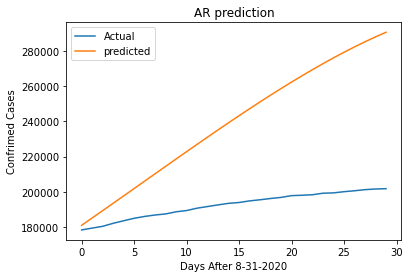
\includegraphics[width=\linewidth]{autoregression.png}
  \caption{Autoregression predictions. Yellow: Actual deaths}
\end{figure}

Due to the lack of generalizability, the Autoregressive Integrated Moving
Average (ARIMA) model was tried, also using the statsmodels module. This model
would use a moving average as well as a linear combination of previous time
steps in order to predict future cases. This of course gave better results
during the validation process, resulting in a validation MAPE of 14.82 for
California. However, the fact that the prediction is linear again resulted in
the same diverging problem as before.

\begin{figure}
  \centering
  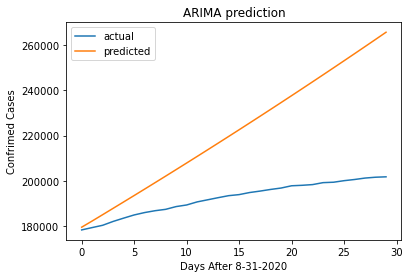
\includegraphics[width=\linewidth]{ARIMA.png}
  \caption{ARIMA: Forecasted Deaths in California}
\end{figure}

From our current progress, we can see that it is hard for the model to take the
plateauing of cases into account. Therefore, we chose to consult the
exponential family of time series models. The exponential family as before uses
a combination of previous times steps to predict future time steps, however, as
the name suggests, this combination is exponentially weighted. What this does
is place more emphasis on the yesterdays cases as opposed to the cases from 4
days ago. This in theory would be more generalizable as we can better locally
approximate changing trends in the data. 

Initially, we used Simple Exponential Smoothing (SES) which was a basic
combination of previous data. SES unfortunately requires the data to not have
any trend which was not the case. This resulted in the model predicting a
constant value leading to a large error. 

Therefore, we used the Holt Winters Exponential Smoothing model which takes
trends into account. While the prediction was still linear, the line was much
closer to the actual number of cases and thus the initial hypothesis of
focusing on recent days to adapt to differing trends indeed turned out to be
true. The validation MAPE for California was around 2.7 which was much better
than our previous models. On the submission data this model scored a 2.28. We
also tried to apply a damping effect to the model and a smoothing factor. Both
resulted in slightly worse performance that the original Holt model, so we
omitted this from our submission.

\begin{figure}
  \centering
  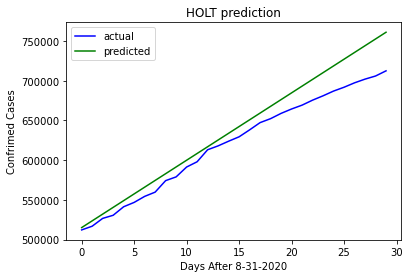
\includegraphics[width=\linewidth]{holt.png}
  \caption{Holt: Predicted Deaths in California}
\end{figure}

\section{Future Plans}

From here on out, we shall focus on decreasing the MAPE score either using
different methods of prediction or by continually extracting features from our
current data or obtaining new types of data within the April - August
timeframe.

\subsection{Preprocessing}

On the data processing side, we also want to consider the utilization of
binning Province\_State values by similarity measures of their Confirmed case
profiles, and work toward integrating the supplemental graph data, namely the
use of the latitude and longitude to establish a physical distance, as well as
the inflow and outflow to cluster states of similar behaviors. We hope that
these efforts would do well to combat potential overfitting to training data
within a state and would encourage a more robust model that can generalize well
to different data.

\subsection{Recurrent Neural Networks}

Our group has also been flirting with the idea of utilizing RNN methods to help
with our forecasting efforts. In pursuing this domain, we will open up the
potential for many more problems with our model architecture and to ensure
correctness of training and implementation, as well as tuning hyperparameters.
We would also need to get the whole group up to speed, which may not be worth
the trouble for something we can’t ensure the success of. We would most likely
employ the use of other methods within the scikit-learn module to integrate
this architecture to our project.
 
It also remains to determine the best method of prediction, as we had initially
misinterpreted the data we would be given for testing – as we now know that we
will only be supplied the Province\_State of interest and the date to be
forecasted. This implies that we will most likely be looking into methods in
which we \emph{a priori} predict functions for each state (or some cluster of
similar states) that predicts cases given the date.


\bibliographystyle{ACM-Reference-Format}
\bibliography{report}

\end{document}
\endinput
